\documentclass[12pt]{article}
\usepackage{graphicx}
\usepackage{wrapfig}
\usepackage{tikz}
\usepackage{ucs} 
\usepackage[T1,T2A]{fontenc}
\usepackage[utf8x]{inputenc} % Включаем поддержку UTF8  
\usepackage[russian]{babel}  % Включаем пакет для поддержки русского языка  
\usepackage{amsfonts}
\usepackage[left=1.5cm,right=1.5cm]{geometry}
\usepackage{amsmath}
\usepackage{amssymb}
\usepackage{xcolor}
\usepackage{hyperref}

% Цвета для гиперссылок
\definecolor{linkcolor}{HTML}{660099} % цвет ссылок
\definecolor{urlcolor}{HTML}{660099} % цвет гиперссылок
\hypersetup{pdfstartview=FitH,  linkcolor=linkcolor,urlcolor=urlcolor, colorlinks=true}

\usetikzlibrary{decorations.markings}
\usetikzlibrary{patterns}
\usetikzlibrary{calc}
\usetikzlibrary{arrows}
\title{Задачи к 5 лекции}  
\author{Нечитаев Дмитрий}

\begin{document} 
	\maketitle
	\section*{Изменения}
	\begin{enumerate}
		\item Новое доказательство максимальности площади в упражнении 2 \hyperref[New proof of task 2]{(ссылка)}
		\item Лагранжиан без первой производной координаты от времени в задаче 2 (ф-ла 2.5.1) \hyperref[Lagrangian]{(ссылка)}
		\item Анализ устойчивости маятника Капицы в задаче 2 \hyperref[Stability analysis]{(ссылка)}
		\item Рассмотрены границы применения потенциала в задаче 2 \hyperref[Resul]{(ссылка)}
		\item Изучение порядка обобщенных скоростей в Лагранжиане \hyperref[Velocities in lagrangian]{(ссылка)}
	\end{enumerate}
	\pagebreak
	\section*{Упражнение 1}
	\subsection*{Лагранжиан в ДСК}
	Выражение для Лагранжиана свободной частицы в интегрциальной системе отсчета с ДПСК:
	\[L = \frac{mv^2}{2} = \frac{m}{2}\big(\dot{x}^2 + \dot{y}^2 + \dot{z}^2\big) \eqno(1)\]
	Находим уравнение движения:
	\[\frac{d}{dt}\frac{\partial L}{\partial \dot{q_i}} = \frac{\partial L}{\partial q_i} \eqno(2)\]
	\[m\ddot{q_i} = 0 \eqno(3)\]
	\subsection*{Лагранжиан в цилиндрических координатах}
	
	\[\begin{cases}
	x = r \cos \phi \\
	y = r \sin \phi \\
	z = z
	\end{cases} \Rightarrow 
	\begin{cases}
	\dot{x} = \dot{r}\cos \phi - r\sin(\phi) \dot{\phi} \\
	\dot{y} = \dot{r}\sin \phi + r\cos(\phi)\dot{\phi} \\
	\dot{z} = \dot{z}
	\end{cases}
	\eqno(4)
	\]
	После возведения в квадрат и подстановки в уравнение (1), получаем:
	\[L = \frac{m}{2}\big( \dot{r}^2+r^2\dot{\phi}^2 + \dot{z} \big) \eqno(5)\]
	Уравнения движения:
	\[\begin{cases}
	m\ddot{r} = mr\dot{\phi}^2 \\
	\frac{d}{dt}\big(mr^2\dot{\phi}^2\big) = 0\\
	m\ddot{z} = 0
	\end{cases} \eqno(6)\]
	\subsection*{Лагранжиан в сферических координатах}
	\[\begin{cases}
	x = r\cos \theta \cos \phi \\
	y = r \cos \theta \sin \phi\\
	z = r \sin \theta
	\end{cases} \Rightarrow 
	\begin{cases}
	\dot{x} = \dot{r}\cos \theta \cos\phi - r\dot{\theta}\sin\theta\cos\phi  - r\dot{\phi}\cos\theta\sin\phi \\
	\dot{y} = \dot{r}\cos \theta \sin\phi - r\dot{\theta}\sin\theta\sin\phi + r\dot{\phi}\cos\theta\cos\phi \\
	\dot{z} = \dot{z}\sin \theta + r\dot{\theta}\cos \theta 
	\end{cases} \eqno(7)\]
	Тогда Лагранжиан примет вид:
	\[L = \frac{m}{2}\big( \dot{r}^2+r^2\dot{\theta}^2 + r^2\dot{\phi}^2\sin^2\theta  \big) \eqno(8)\]
	Уравнения движения:
	\[\begin{cases}
	m\ddot{r} =  mr\dot{\theta}^2 + mr\dot{\phi}^2\sin^2\theta\\
	\frac{d}{dt}\big(mr^2\dot{\theta}\big) = mr^2\dot{\phi}^2\sin(\theta)\cos(\theta) \\
	\frac{d}{dt}\big(mr^2\sin^2(\theta)\dot{\phi}\big) = 0
	
	\end{cases} \eqno(9)\]
	
	\subsection*{Лагранжиан в криволиниейных координатах}
	Пусть нам теперь дан закон преобразования координат:
	\[\begin{cases}
	x = x(\xi,\eta,\zeta) \\
	y = y(\xi,\eta,\zeta) \\
	z = z(\xi,\eta,\zeta) \\
	\end{cases} \Rightarrow D = \begin{pmatrix}
	\partial x / \partial \xi && \partial x / \partial \eta && \partial x / \partial \zeta \\
	\partial y / \partial \xi && \partial y / \partial \eta && \partial y / \partial \zeta \\
	\partial z / \partial \xi && \partial z / \partial \eta && \partial z / \partial \zeta \\
	\end{pmatrix} \eqno(10)\]
	Тогда справедливо соотношение между дифференциалами:
	\[\begin{pmatrix}
	dx \\ dy \\ dz
	\end{pmatrix} = D \begin{pmatrix}
	d\xi \\ d\eta \\ d\zeta
	\end{pmatrix} \Rightarrow 
	\begin{pmatrix}
	dx & dy & dz 
	\end{pmatrix} = 
	\begin{pmatrix}
	d\xi &  d\eta & d\zeta
	\end{pmatrix} D^T \eqno(11)\]
	Перемножая строчку и столбец можно определить выражение для $dl^2$:
	\[dl^2 = \begin{pmatrix}dx & dy & dz\end{pmatrix} \begin{pmatrix}dx \\ dy \\dz \end{pmatrix} = \begin{pmatrix} d\xi &  d\eta & d\zeta \end{pmatrix} D^T D \begin{pmatrix}
	d\xi \\ d\eta \\ d\zeta
	\end{pmatrix} \eqno(12)\]
	Замечаем, что $v^2dt^2 = dl^2$, т.е Лагранжиан преобретает вид:
	\[L = \frac{m}{2} \begin{pmatrix} \dot{\xi} &  \dot{\eta} & \dot{\zeta} \end{pmatrix} D^T D \begin{pmatrix}\dot{\xi} \\  \dot{\eta} \\ \dot{\zeta} \end{pmatrix} \eqno(13)\]	
	Пусть $\{q_1,q_2,q_3\}$ - новые координаты, а $\{x_1,x_2,x_3\}$ - старые координаты, тогда:
	\[D = \Big(\frac{\partial x^i}{\partial q^j}\Big) \Rightarrow L = \frac{m}{2}\Big(\dot{q}^j\frac{\partial x^i}{\partial q^j}\frac{\partial x^i}{\partial q^k} \dot{q}^k \Big) = \frac{m}{2}\Big(\dot{q}^j\dot{q}^k\frac{\partial x^i}{\partial q^j}\frac{\partial x^i}{\partial q^k} \Big) \eqno(14)\]
	Из выражения (14) можно получить, что в Лагранжиан обобщенные скорости входят только во второй степени, данные рассуждения работают, если нет зависимости координатных функций от времени, в противном случае появляются дополнительные слагаемые.
	
	
	Получим уравнения движения. Для этого продифференцируем Лагранжиан по $\dot{q}^p$:
	\[\frac{\partial L}{\partial \dot{q}^p} = \frac{m}{2}\Big( \delta^j_p \dot{q}^k\frac{\partial x^i}{\partial q^j}\frac{\partial x^i}{\partial q^k} + \delta^k_p \dot{q}^j\frac{\partial x^i}{\partial q^j}\frac{\partial x^i}{\partial q^k} \Big) = m\dot{q}^k \frac{\partial x^i}{\partial q^p}\frac{\partial x^i}{\partial q^k} \eqno(15) \]
	Тогда уравнения движения принимают вид:
	\[\frac{d}{dt}\Big( m\dot{q}^k \frac{\partial x^i}{\partial q^p}\frac{\partial x^i}{\partial q^k} \Big) = \frac{\partial }{\partial q^p} \Big( \frac{m}{2}\dot{q}^j\dot{q}^k\frac{\partial x^i}{\partial q^j}\frac{\partial x^i}{\partial q^k} \Big) \eqno(16)\]
	\subsection*{Криволинейные координаты с зависимостью от времени}\label{Velocities in lagrangian}
	Выясним что происходит с Лагранжианом, когда координатные функции зависят от времени. Пусть $\{q_1,q_2,q_3\}$ - новые координаты, а $\{x_1,x_2,x_3\}$ - старые координаты, тогда:
	\[v^2 = \frac{dx^i}{dt}\cdot\frac{dx^i}{dt} = \Big(\frac{\partial x^i}{\partial q^j}\dot{q}^j+\frac{\partial x^i}{\partial t}\Big)\Big(\frac{\partial x^i}{\partial q^k}\dot{q}^k+\frac{\partial x^i}{\partial t}\Big) = \dot{q}^k\dot{q}^j\frac{\partial x^i}{\partial q^k}\frac{\partial x^i}{\partial q^j} + 2\dot{q^k}\frac{\partial x^i}{\partial q^k}\frac{\partial x^i}{\partial t} + \frac{\partial x^i}{\partial t}\cdot\frac{\partial x^i}{\partial t} \eqno(17)\]
	Первый член характеризует относительное изменение координаты частицы, а два последних учитывают движение системы координат. Лагранжиан примет вид:
	\[L = \frac{m}{2}\Big(\dot{q}^k\dot{q}^j\frac{\partial x^i}{\partial q^k}\frac{\partial x^i}{\partial q^j} + 2\dot{q^k}\frac{\partial x^i}{\partial q^k}\frac{\partial x^i}{\partial t} + \frac{\partial x^i}{\partial t}\cdot\frac{\partial x^i}{\partial t}\Big) \eqno(18)\]
	В качестве примера, когда в Лагранжиане есть слагаемое, содержащее первую степень скорости, можно взять с/к, которая движется равноускоренно вдоль оси $OX$.
	\[L = \frac{m}{2}\Big(v^2_\text{отн}+2v_\text{отн}at+a^2t^2\Big) \eqno(19)\]
	Получается, что если координатные функции не содержат зависимости от $t$, то Лагранжиан свободной частицы имеет только члены квадратичные по скоростям. Если зависимость от времени присутствует, то могут появиться члены первого порядка.
	 
	
	\section*{Упражнение 2}
	\subsection*{Поиск решения}
	Пусть дана гладкая замкнутая кривая $\Gamma$ без самопересечений.Необходимо найти кривую, которая при заданной длине ограничивает максимальную площадь.
	
	Для решения введем 2 интегральных представления: площади $A$ и длины $P$, задаваемые следующими формулами:
	\[A[\Gamma] = \int_{S} dxdy = \frac{1}{2}\int_{\Gamma} xdy - ydx = \frac{1}{2} \int_{0}^{1} (x\dot{y} - y\dot{x})dt \eqno(1)\]
	\[P[\Gamma] = \int_{0}^{1} \sqrt{\dot{x}^2+\dot{y}^2} ds \eqno(2)\]
	Если зафиксировать длину кривой, но изменять площадь, то получим задачу на условный экстремум функционала $A[\Gamma]$, причем т.к условие записано в интегральном представлении, то для нахождения нужной кривой достаточно исследовать на безусловный экстремум функционал:
	\[F[\Gamma](\lambda) = A[\Gamma] - \lambda P[\Gamma] = \int_{0}^{1} \Big(\frac{1}{2}(x\dot{y}-y\dot{x}) - \lambda\sqrt{\dot{x}^2+\dot{y}^2}\Big)dt\;\;\;\text{где $\lambda \in \mathbb{R}$} \eqno(3)\]
	Для этого воспользуемся уравнение Эйлера-Лагранжа:
	\[
	\frac{\partial L}{\partial q_i} = \frac{d}{dt}\frac{\partial L}{\partial \dot{q_i}} \Leftrightarrow
	\begin{cases}
	\frac{1}{2}\dot{y} = \frac{d}{dt}\Big( -\frac{y}{2} - \frac{\lambda\dot{x}}{\sqrt{\dot{x}^2 + \dot{y}^2}} \Big) \\
	-\frac{1}{2}\dot{x} = \frac{d}{dt}\Big( \frac{x}{2} - \frac{\lambda\dot{x}}{\sqrt{\dot{x}^2 + \dot{y}^2}} \Big)
	\end{cases} \Leftrightarrow 
	\begin{cases}
	\frac{d}{dt}\Big( y + \frac{\lambda\dot{x}}{\sqrt{\dot{x}^2 + \dot{y}^2}} \Big) = 0 \\
	\frac{d}{dt}\Big( x - \frac{\lambda\dot{x}}{\sqrt{\dot{x}^2 + \dot{y}^2}} \Big) = 0
	\end{cases} \eqno(4)\]
	Из системы следует, что выражения под знаком дифференциала сохраняются, т.е. являются константами:

	
	\[\begin{cases}
	y + \frac{\lambda\dot{x}}{\sqrt{\dot{x}^2 + \dot{y}^2}} = C_1 \\
	x - \frac{\lambda\dot{x}}{\sqrt{\dot{x}^2 + \dot{y}^2}} = C_2		
	\end{cases} \Leftrightarrow 
	\begin{cases}
	C_1 - y = \frac{\lambda\dot{x}}{\sqrt{\dot{x}^2 + \dot{y}^2}}\\
	x - C_2 = \frac{\lambda\dot{x}}{\sqrt{\dot{x}^2 + \dot{y}^2}}
	\end{cases} \Rightarrow (x-C_1)^2+(y-C_2)^2 = \lambda^2 \eqno(5)\]
	  
	Получилось уравнение окружности, причем константу $\lambda$ можно найти из условия для периметра $\pm2\pi \lambda = P$, тогда все потенциально подходящие кривые описываются уравнением:
	\[\boxed{(x-C_1)^2+(y-C_2)^2 = \frac{P^2}{4\pi^2}} \eqno(6)\]
	
		\subsection*{Доказательство максимальности} \label{New proof of task 2}
	
	Перепишем функционал $F[\Gamma]$ в полярных координатах:
	\[F[\Gamma](\lambda) = \int_0^{2\pi}\Big(\frac{1}{2}r^2 - \lambda \sqrt{r^2+r'^2}\Big)d\phi \eqno(7)\]
	Переобозначим подынтегральную функцию как $L(r,r',\phi)$, тогда вторая вариационная производная $F[\Gamma](\lambda)$ в точке $r(\phi) = r_0 $, где $r_0$ --- радиус окружности.
	\[\frac{\delta^2F}{\delta\eta^2} = \lim\limits_{\alpha \rightarrow 0} \frac{\partial^2 }{\partial \alpha^2} \int_0^{2\pi} L (r_0+\alpha\eta,r_0'+\alpha\eta',\phi)d\phi = \int_0^{2\pi} \lim\limits_{\alpha \rightarrow 0} \frac{\partial^2 }{\partial \alpha^2} L (r_0+\alpha\eta,r_0'+\alpha\eta',\phi)d\phi \eqno(8)\]
	Для нахождения втой производной посчитаем $d^2L$, с учетом того, что функция не зависит явно от $\phi$ получаем соотношение:
	\[d^2L = \frac{\partial^2 L}{\partial r^2 }dr^2 +  \frac{\partial^2 L}{\partial r'^2 } dr'^2 + 2 \frac{\partial^2 L}{\partial r\partial r' }dr'dr \eqno(9)\]
	Непосредственное вычисление частных производных и подстановка функции $r(\phi) = r_0 = const$
	
	\[
	\large
	\begin{cases}
		\frac{\partial^2 L}{\partial r^2 } = 1 - \lambda\frac{r'^2}{(r^2+r'^2)^{3/2}} \\
		\frac{\partial^2 L}{\partial r'^2 } = - \lambda\frac{r^2}{(r^2+r'^2)^{3/2}} \\
		\frac{\partial^2 L}{\partial r \partial r' } = \lambda \frac{rr'}{(r^2+r'^2)^{3/2}}
	\end{cases} \Rightarrow
	\begin{cases}
		\frac{\partial^2 L}{\partial r^2 } = 1 \\
		\frac{\partial^2 L}{\partial r'^2 } = - \frac{\lambda}{r_0} \\
		\frac{\partial^2 L}{\partial r \partial r' } = 0
	\end{cases}
	\normalsize
	\eqno(10)\]
	Вместо $dr$ подставляем $\alpha \eta$, а $dr'$ заменяем на $\alpha\eta'$, тогда вторая вариационная производная примет вид\footnote{Тут мы подставили значение $dr,dr'$, затем использовали формулу Тейлора $L(q,q',t) = L(q_0,q_0',t)+dL + \frac{1}{2!}d^2L + ... $, вычислили производную по $\alpha$, затем взяли предел.}:
	\[\frac{\delta^2F}{\delta\eta^2} = \int_0^{2\pi}\Big(\eta^2 - \frac{\lambda}{r_0}\eta'^2\Big)d\phi \eqno(11)\]
	Вспомним, что из условия на периметр было получено: $\lambda = r_0 $.
	\[\frac{\delta^2F}{\delta\eta^2} = \int_0^{2\pi}\Big(\eta^2 - \eta'^2\Big)d\phi \eqno(12)\]
	Тут $\eta$ - хорошая\footnote{Суммируемая с квадратом на $\left[0;2\pi\right]$, дифференцируемая.} периодическая функция, которую можно разложить в ряд Фурье:
	\[\eta = \sum_{n = 1}^{\infty} A_n \sin(n\phi)+B_n\cos(n\phi) \Rightarrow \eta' = \sum_{n = 1}^{\infty} A_n n \cos(n\phi)-B_n n \sin(n\phi) \eqno(13)\]
	Тогда равенство Парсеваля дает:
	\[\sum_{n = 1}^{\infty} A_n^2 + B^2_n - n^2A_n^2 - n^2B^2_n = \frac{1}{\pi}\int_0^{2\pi}\Big(\eta^2 - \eta'^2\Big)d\phi \eqno(14)\]
	Левая часть уравнения (14) отрицательна, при всех функциях $\eta \in C^1[0;2\pi]$, кроме функций вида: $A\sin(\phi)+B\cos(\phi)$. Покажем, что класс подобных функций периметр не сохраняет.
	
	
	
	Несколько рассуждений позволят нам упростить дальнейшие выкладки:
	\begin{enumerate}
		\item Функцию вида $A\sin\phi + B\cos\phi$ можно привести к виду $R\sin(\phi+\theta)$, где $R,\theta \in \mathbb{R}$
		\item Т.к. мы будем производить интегрирование по периоду, то на $\theta$ можно не обращать внимание.
	\end{enumerate}
	С учетом сказанного выше находим периметр:
	\[\tilde{P} = \int_0^{2\pi}\sqrt{(r_0+R\sin\phi)^2 + R^2\cos^2\phi}d\phi = \int_0^{2\pi}\sqrt{r_0^2 + 2r_0R\sin\phi + R^2}d\phi \eqno(15)\]
	Эллиптический интеграл, брать мы, конечно, не будем, а вот оценить разность можно.
	\[\tilde{P} - P =\int_0^{\pi}\Big(\sqrt{r_0^2 + 2r_0R\sin\phi + R^2} - r_0\Big)d\phi + \int_0^{\pi}\Big(\sqrt{r_0^2 - 2r_0R\sin\phi + R^2}-r_0\Big)d\phi \eqno(16) \]
	Покажем, что периметр $\tilde{P}$ будет больше изначального периметра. Для этого исследуем на сколько сильно отличаются подынтегральные выражения от $r_0$.
	\[\sqrt{r_0^2+R^2+2r_0R\sin\phi} - r_0 \;\;\vee \;\;r_0 - \sqrt{r_0^2+R^2-2r_0R\sin\phi} \]
	\[\sqrt{r_0^2+R^2+2r_0R\sin\phi} + \sqrt{r_0^2+R^2-2r_0R\sin\phi} \;\;\vee \;\; 2r_0\]
	\[2r_0^2+2R^2 + 2\sqrt{(r_0^2+R^2)^2-4r_0^2R^2\sin^2\phi} \;\;\vee \;\; 4r_0^2\]
	\[\sqrt{(r_0^2+R^2)^2-4r_0^2R^2\sin^2\phi} \;\; \vee \;\; r_0^2-R^2 > 0\]
	\[r_0^4+R^4+2r_0^2R^2 - 4r_0^2R^2\sin^2\phi \;\;\vee\;\; r_0^4+R^4-2r_0^2R^2\]
	\[r_0^2R^2 \vee r_0^2R^2\sin^2\phi\]
	\[1 \vee \sin^2\phi\]
	\[1 \ge \sin^2\phi\]
	\begin{figure}[h!]
		\center{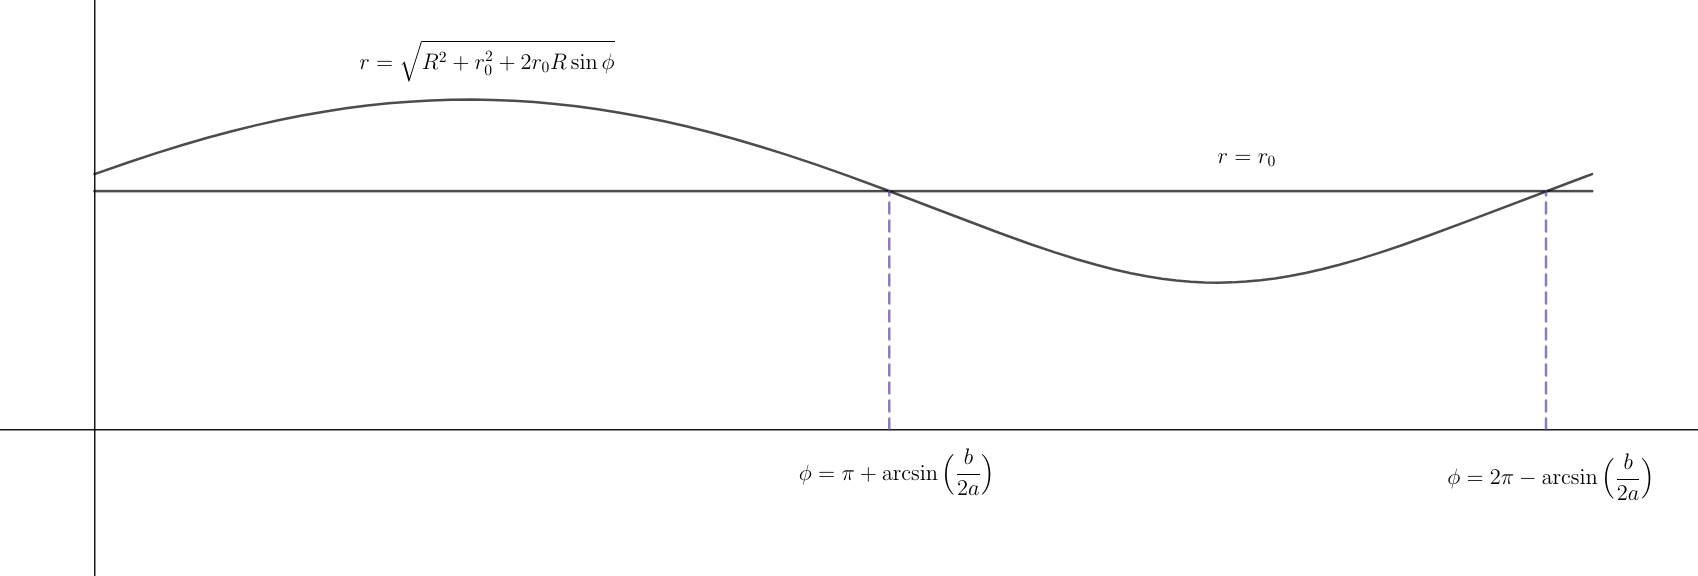
\includegraphics[scale=0.4]{sketch.png}}
	\end{figure}
	
	
	Данная цепочка сравнений справедлива при двух словиях: $r_0>R$ и $x \in \left[\arcsin(\frac{R}{2r_0});\pi-\arcsin(\frac{R}{2r_0})\right]$.
	Второе условие отвечает тому, что $r_0-\sqrt{r_0^2+R^2-2r_0R\sin\phi} \ge 0$.
	
	
	
	Возвращаясь к интегралу (16) делаем вывод, что на $x \in \left[\arcsin(\frac{b}{2a});\pi-\arcsin(\frac{b}{2a})\right]$ сумма от двух интегралов положительна. На оставшемся множестве подынтегральные функции положительны, а значит и разность периметров не будет равна 0.
	
	
	Таким образом мы доказали, что семейство возмущений $\eta = A\sin\phi + B\sin\phi$ при достаточно малых $\sqrt{A^2+B^2}$ не входит во множество функций, которые сохраняют периметр фигуры. Таким образом доказан сильный максимум функционала $F[\Gamma]$.
	
	
	
	
	\section*{Задача 1}
	Пусть дан шарик и две точки в пространстве с известными координатами. Какую форму желоба нужно сделать, чтобы шарик без начальной скорости скатился под действием силы тяжести от одной точки к другой за наименьшее время?
	
	
	Для удобства введем систему координат как показано на рисунке:
	\begin{figure}[h!]
		\center{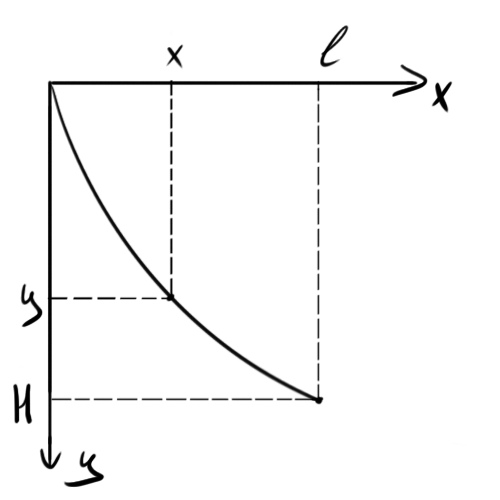
\includegraphics[scale=0.5]{task2_system.jpg}}
	\end{figure}
	Пусть параметризация кривой имеет вид: $y = y(x)$, тогда длина элемента дуги определяется соотношением:
	\[dl = \sqrt{1+y'^2}dx \eqno(1)\]
	Из теоремы об изменении кин энергии находим:
	\[ v = \sqrt{\varkappa y} \eqno(2)\]
	Тогда за время $dt = dl / v$ шарик пройдет кусочек дуги, а значит для оптимизации времени спуска можно ввести функционал:
	\[S[y(x)] = \int_{0}^{l} \frac{\sqrt{1+y'^2}}{\sqrt{\varkappa y}} dx \eqno(2)\]
	Для удобства рассчетов таскать за собой $\sqrt{\varkappa}$ не будем. Обозначим подынтегральное выражение за $L(y,y')$.
	
	Можно и дальше упрощать жизнь: для этого стоит заметить, что $L$ не зависит явно от $x$, а это нам очень помогает, ведь тогда верен переход:
	\[\frac{dL}{dx} = \frac{\partial L}{\partial y} y' + \frac{\partial L}{\partial y'} y'' + \frac{\partial L}{\partial x}\;\;\; \Leftrightarrow\;\;\; \frac{dL}{dx} = \frac{\partial L}{\partial y} y' + \frac{\partial L}{\partial y'} y'' \;\;\; \Leftrightarrow \;\;\; \frac{\partial L}{\partial y} y' = \frac{dL}{dx} - \frac{\partial L}{\partial y'} y'' \eqno(3)\]
	Для оптимизации интегрального функционала используем уравнение Эйлера-Лагранжа:
	\[\frac{\partial L}{\partial y} = \frac{d}{dx} \frac{\partial L}{\partial y'} \eqno(4)\]
	Домножим обе части на $y'$ и воспользуемся подстановкой из выражения (3):
	\[\frac{dL}{dx} = y''\frac{\partial L}{\partial y'} + y' \frac{d}{dx} \frac{\partial L}{\partial y'} = \frac{d}{dx}\Big( y' \frac{\partial L}{\partial y'}\Big) \;\; \Leftrightarrow \;\; \frac{d}{dx}\Big(L - y' \frac{\partial L}{\partial y'} \Big) = 0 \eqno(5)\]
	Поучаем дифференциальное уравнение:
	\[L - y' \frac{\partial L}{\partial y'} = C \eqno(6)\]
	Подставляем $L$ в уравнение (6):
	\[\frac{\sqrt{1+y'^2}}{\sqrt{y}} - y' \frac{y'}{\sqrt{y}\sqrt{1+y'^2}} = C\;\; \Leftrightarrow \;\; \frac{1}{\sqrt{y}\sqrt{1+y'^2}}=C \;\; \Leftrightarrow \;\; (1+y'^2)y = (1/C)^2 \equiv k \eqno(7)\]
	\[y'^2 = \frac{k}{y}-1 \;\; \Rightarrow \;\; y' = \sqrt{\frac{k-y}{y}} \Leftrightarrow \sqrt{\frac{y}{k-y}} dy = dx \eqno(8)\]
	\[y = k\sin^2 \theta \Rightarrow dy = 2k\sin \theta \cos \theta d\theta  \eqno(9)\]
	\[\int_{0}^{\theta_0} \Big|\frac{\sin\theta}{\cos \theta}\Big| 2k \cos \theta \sin \theta d \theta = k \int_{0}^{\theta_0}(1-\cos(2\theta)) d\theta = \frac{k}{2}\Big(2\theta_0 - \sin(2\theta_0)\Big) = x(\theta_0) \eqno(10)\]
	Получаем кривую, заданную параметрически:
	\[\boxed{
	\begin{cases}
	x(\theta) = \frac{k}{2}\Big(2\theta - \sin(2\theta)\Big) \\
	y(\theta) = k\sin^2(\theta)
	\end{cases} \forall \theta \in \left[0;\frac{\pi}{2}\right]}\eqno(11)\]
	Числа $k,\theta_0$ находится из системы (11) при подстановке $x(\theta_0) = l$ и $y(\theta_0) = H$.
	

	\pagebreak
	\section*{Задача 2}
	Рассмотрим обычный маятник, точка подвеса которого может совершать движение по какому-то произвольному, но известному закону $\textbf{r}(t)$. Сам маятник представляет собой невесомую палку длины $l$ и с массой $m$ на конце.
	\subsection*{1. Лагранжиан системы}
	Для однозначного определения положения маятника нам достаточно знать где находится точка подвеса и 2 угла, задающие точку на сфере, причем скорость маятника определяется соотношением:
	\[\vec{V_A} = \vec{V_0} + \vec{\omega}\times \vec{l} \eqno(1.1)\]
	\begin{figure}[h!]
		\center{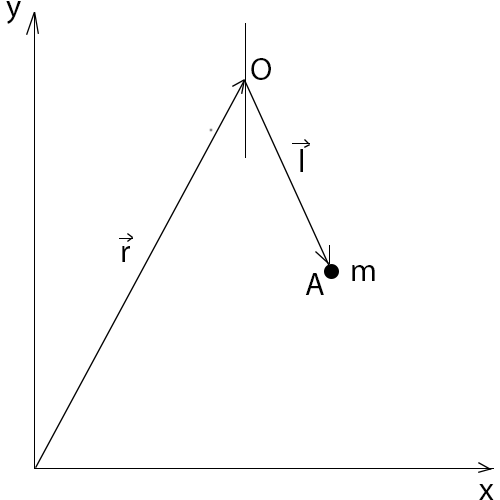
\includegraphics[scale=0.5]{pendulum.png}}
	\end{figure}


	Тогда лагранжиан системы примет вид:
	\[L = \frac{m(\vec{V_0}(t) + \vec{\omega}\times \vec{l})^2}{2} + m\vec{g}\Big(\;\vec{r}(t)+\vec{l}\;\Big) \eqno(1.2)\]
	\[L = \frac{m}{2}V_0^2 + \frac{m}{2}\omega^2 l^2 + m(\vec{V_0},\vec{\omega} \times \vec{l}) + m\vec{g}\Big(\;\vec{r}+\vec{l}\;\Big) \eqno(1.3)\]

	\subsection*{2. Конкретный закон $r(t)$}
	Пусть теперь $\vec{r}(t) = r_0 \cos (\gamma t) \cdot (\cos \theta,\sin \theta)$, тогда лагранжиан примет вид:
	\[L = \frac{m}{2} \gamma ^2 r_0^2 \sin^2(\gamma t) + \frac{m}{2}\dot{\phi}^2 l ^2 - m \gamma r_0 \sin(\gamma t) \dot{\phi} l \cos(\phi - \theta) - mg\Big( r_0 \cos(\gamma t) \sin(\theta) - l\cos(\phi) \Big) \eqno(2.1) \]
	
	\begin{figure}[h!]
		\center{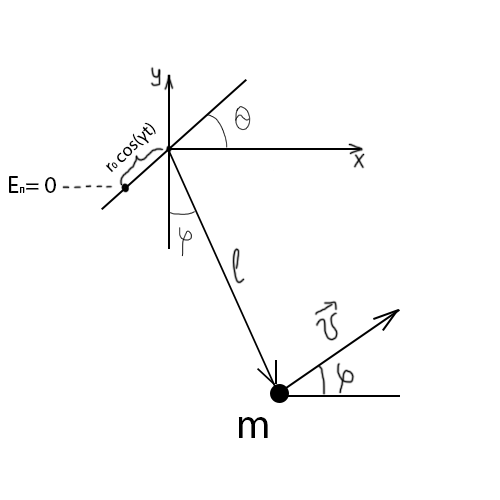
\includegraphics[scale=0.5]{pendulum_k.png}}
	\end{figure}


	Выкидываем все полные производные из Лагранжиана:
	\[L = \frac{m}{2}\dot{\phi}^2l^2 -  m \gamma r_0 \sin(\gamma t) \dot{\phi} l \cos(\phi - \theta) +mgl\cos(\phi) \eqno(2.2)\]
	Если ввести обозначения $\tau = \omega_0 t$, $\omega_0 = \sqrt{g/l}$, $A = \frac{\gamma}{\omega_0}\frac{r_0}{l}$, $B = \frac{\gamma}{\omega_0}$ то можно обезразмерить Лагранжиан ($m=1$):
	\[\tilde L = \frac{\dot{\phi}^2}{2\omega_0^2}-A\frac{\dot{\phi}}{\omega_0}\sin(\gamma t)\cos(\phi-\theta) + \cos(\phi) \eqno(2.3)\]
	Параметр $A$ характеризует отношение максимальных скоростей точки подвеса $(\gamma r_0)$ и математического маятника $(\omega_0 l)$. Последним штрихом будет нахождение связи между производными $\phi'_\tau$ и $\phi'_t$:
	\[\frac{d\phi}{dt} = \frac{d\phi}{d\tau} \frac{d\tau}{dt} \Leftrightarrow \frac{\phi'_t}{\omega_0} = \phi'_\tau \eqno(2.4)\] 
	Собираем все вместе:
	\[ \tilde L =  \frac{{\phi'}_{\tau}^2}{2} - A\phi'_\tau\sin(B \tau)\cos(\phi-\theta) + \cos(\phi) \eqno(2.5)\]
	Выделим полную производную по времени:
	\[\tilde{L} = \frac{{\phi'}_{\tau}^2}{2} + \cos(\phi) + \Big(- A\phi'_\tau\sin(B \tau)\cos(\phi-\theta) - B\cos(B\tau)A\sin(\phi-\theta)\Big) + B\cos(B\tau)A\sin(\phi-\theta) = \]
	\[= \frac{{\phi'}_{\tau}^2}{2} + \cos(\phi) + \frac{d}{d\tau}\Big(- A\sin(B \tau)\sin(\phi-\theta)\Big) + AB\cos(B\tau)\sin(\phi-\theta) \]
	Выкидываем полную производную:
	\[\tilde{L} = \frac{{\phi'}_{\tau}^2}{2} + \cos(\phi) + AB\cos(B\tau)\sin(\phi-\theta) \eqno(2.5.1)\label{Lagrangian}\]
	Находим уравнения движения:
	\[ \frac{d}{d\tau}\Big(\phi'_\tau - A\sin(B \tau)\cos(\phi-\theta) \Big) = -A\phi'_\tau\sin(B \tau)\sin(\phi-\theta) - \sin(\phi) \Leftrightarrow \]
	\[ \phi''_\tau + A\phi'_\tau\sin(B \tau)\sin(\phi-\theta) - AB\cos(B\tau)\cos(\phi-\theta) = A\phi'_\tau\sin(B \tau)\sin(\phi-\theta) - \sin(\phi) \Leftrightarrow \]
	\[ \phi''_\tau = AB\cos(B\tau)\cos(\phi-\theta)-\sin(\phi) \eqno(2.6)\]
	Или в старых обозначениях:
	\[\ddot{\phi}+\omega_0^2\sin(\phi) = \frac{r_0}{l}\gamma^2 \cos(\gamma t) \cos(\phi-\theta) \eqno(2.7)\]
	\subsection*{3. Вспомогательная задача}
	
	
	Рассмотрим колебание грузика на пружинке жесткости $k$, к которому приложена быстрая периодическая сила $F = mf_0 \cos(\omega t)$,  $\omega \gg \sqrt{k/m}=\omega_0$.
	
	
	Уравнение движения:
	\[x'' + \omega_0^2 x = f_0 \cos(\omega t)\;\;\;x(0)=0,\;\;\;x'(0)=v_0 \eqno(3.1)\]
	Точное решение данной задачи Коши:
	\[x(t) = \frac{f_0}{\omega^2-\omega_0^2}\cos(\omega_0 t)+\frac{f_0}{\omega_0^2-\omega^2}\cos(\omega t) + \frac{v_0}{\omega_0}\sin(\omega_0 t) \eqno(3.2)\]
	\begin{figure}[h!]
		\center{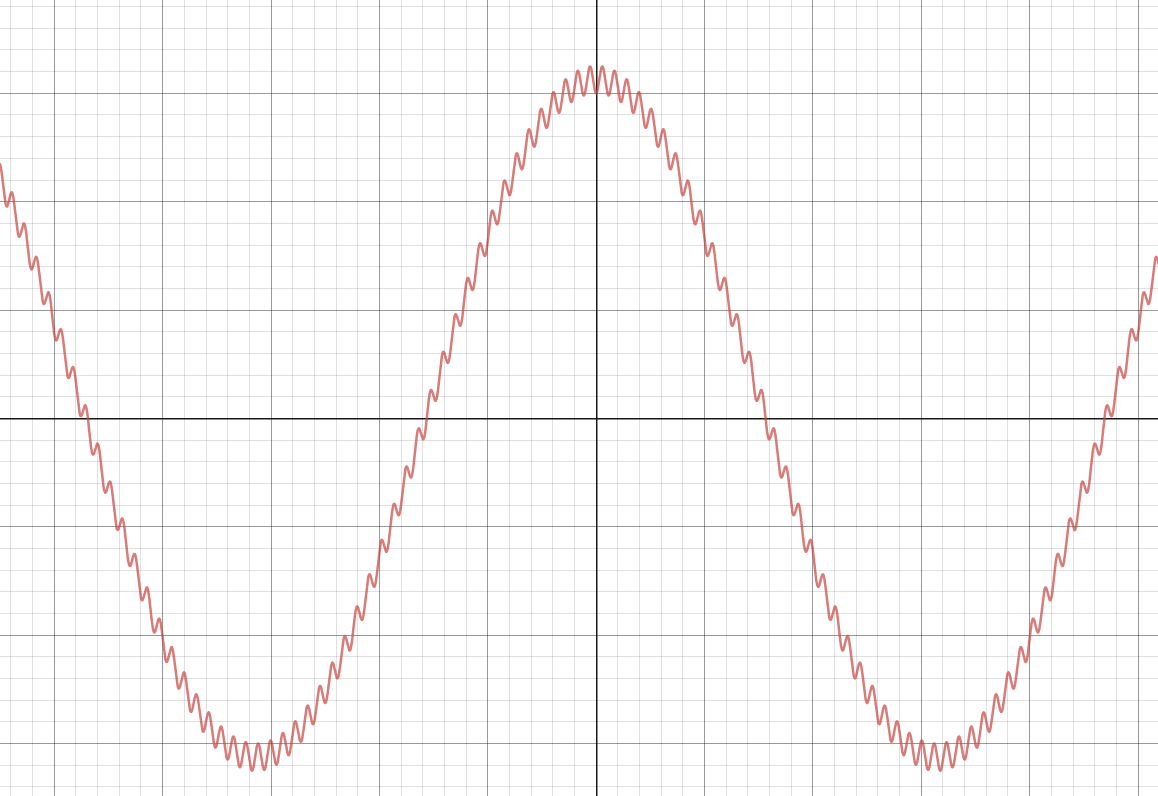
\includegraphics[scale=0.25]{solution_pendulum.png}}
		\caption{График решения $x(t)$ при $\omega/\omega_0 = 55$   }
	\end{figure}
	
	\pagebreak
	Перепишем уравнение (3.2) и учтем, что $v_0/\omega_0 \gg f_0 / (\omega^2-\omega^2_0)$, при $\omega \gg \omega_0$:
	\[x(t) \approx \frac{f_0}{\omega_0^2-\omega^2}\cos(\omega t) + \frac{v_0}{\omega_0}\sin(\omega_0 t) \eqno(3.3)\]
	Вид уравнения (3.3) позволяет сделать некоторые выводы относительно решения:
	\begin{enumerate} 
		\item В системе есть 2 характерных времени $\tau_1 = 1/\omega_0$ и $\tau_2 = 1/\omega$. Это связано с тем, что решение уравнения состоит из двух гармоник. Гармоника с частотой $\omega_0$ отвечает за движение маятника без учета внешней силы: $x_0(t)$ --- невозмущенное решение. Вторая гармоника задает смещение относительно $x_1(t)$ и появляется из-за внешней силы.
		\item Смещение относительно невозмущенного решения задается формулой:
		\[x_1(t) = \frac{f_0}{\omega_0^2-\omega^2}\cos(\omega t) \eqno(3.4)\]
		При $\omega \gg \omega_0$ можно разложить $x_1(t)$ по степеням $\omega_0 /\omega$. Первый порядок дает нам ответ:
		\[x_1(t) \approx -\frac{f_0}{\omega^2}\cos(\omega t ) \eqno(3.5)\]
	\end{enumerate}

	\subsection*{4. Быстрые и медленные переменные}
	Вернемся к исследованию решения уравнения (2.7). Решение будем искать в виде суммы $\phi(t) = \psi(t)+\chi(t)$, где $\psi(t)$ --- периодическое решение с частотой $\omega_0$, а $\chi(t)$ --- периодическое решение с частотой $\gamma$ и амплитудой $ \ll 1$.
	
	
	Малось амплитуды решения с частотой $\gamma$ следует из соотношения (3.5). Действительно, если подставить в качестве $f_0 = \frac{r_0}{l} \gamma^2 cos(\phi-\theta)$, то амплитуда $\chi$ будет порядка $r_0/l \ll 1$.
	
	Подставим теперь в уравнение (2.7) вместо $\phi(t)$ сумму $\psi(t)+\chi(t)$, раскладывая функции по степеням $\chi$ до первого порядка.
	\[\ddot{\psi}+\ddot{\chi} + \omega_0^2\sin\psi + \chi \omega_0^2 \cos \psi = \frac{r_0}{l}\gamma^2\cos(\gamma t)\Big(\cos(\psi-\theta)-\chi\sin(\psi-\theta)\Big) \eqno(4.1)\]
	Т.к функция $\chi(t)$ осциллирует с частотой $\gamma$, то для получения уравения на $\chi(t)$ необходимо сгруппировать все слагаемые осциллирующие с той же частотой (или достаточно близкой к ней).
	\[\ddot{\chi} + \chi \omega_0^2 \cos \psi = \frac{r_0}{l}\gamma^2\cos(\gamma t)\Big(\cos(\psi-\theta)-\chi\sin(\psi-\theta)\Big) \eqno(4.2)\]
	Теперь вспоминаем, что на самом деле $\chi \ll 1$ и слагаемые содержащие $\chi$ можно выкинуть. Но выкидывать $\ddot{\chi}$ \textbf{НЕЛЬЗЯ} т.к. амплитуда второй производной порядка $\frac{r_0}{l}\gamma^2 \gg \frac{r_0}{l}$.
	\[\ddot{\chi} = \frac{r_0}{l}\gamma^2\cos(\gamma t)\cos(\psi - \theta) \Rightarrow \chi(t) = -\frac{r_0}{l}\cos(\gamma t)\cos(\psi - \theta)\eqno(4.3)\]
	В последнем переходе мы интегрировали вторую производную, считая что $\psi$ на временах порядка $1/\gamma$ практически не меняется.
	
	Усредним уравнение (4.1) по периоду $T = 2\pi/\gamma$, в таком случае все слагаемые содержащие $\chi$ в нечетных степенях обратятся в 0, а величины, которые осциллируют с частотой $\omega_0 \ll \gamma$ практически не изменяются.
	\[\ddot{\psi} + \omega_0^2 \sin\psi  = \frac{r_0^2\gamma^2}{l^2} <\cos^2(\gamma t)>_T \sin(\psi-\theta)\cos(\psi-\theta) = \frac{r_0^2\gamma^2}{2l^2}\sin(\psi-\theta)\cos(\psi-\theta) \eqno(4.4)\]
	
	Преобразуем выражение:
	\[\ddot{\psi} = -\frac{d}{d\psi}\Bigg( \frac{r_0^2\gamma^2}{4l^2}\cos^2(\psi-\theta) - \omega_0^2\cos\psi  \Bigg)\eqno(4.5)\]
 	Выражение в скобках можно заменить функцией $U_{\text{эфф}}(\psi)$.
 	\[U_{\text{эфф}}(\psi) = \frac{r_0^2\gamma^2}{4l^2}\cos^2(\psi-\theta) - \omega_0^2\cos\psi \eqno(4.6)\]
 	
 	\pagebreak
 	\subsection*{5. Положения равновесия и их устойчивость}
 	\subsubsection*{1 случай $\theta = \frac{\pi}{2}$} 
 	Положения равновесия соответствуют экстремумам потенциалной энергии. Используем коэффециент $A$, введенный во 2 пункте, тогда при $\theta = \pi/2$ потенциал можно переписать:
 	\[U = \omega_0^2\Big(\frac{A^2}{4}\sin^2(\psi)-\cos(\psi)\Big) \eqno(5.1.1)\]
 	\[\frac{dU}{d\psi} = \omega_0^2 \Big(\frac{A^2}{2}\sin\psi\cos\psi + \sin\psi \Big) \eqno(5.1.2)\]
 	\[\frac{d^2U}{d\psi^2} = \omega_0^2 \Big(\frac{A^2}{2}\cos(2\psi) + \cos\psi \Big) \eqno(5.1.3)\]
 	Точки экстремума отвечают углам: $0,\;\pi,\;\arccos(-2A^{-2})$, причем положение $\psi = 0$ устойчиво, а $\psi = \arccos(-2A^{-2})$ устойчивым не является:
 	\[\frac{d^2U}{d\psi^2} (\arccos(-2A^{-2})) = \omega_0^2 \Big(\frac{A^2}{2}(2(2A^{-2})^{2}-1) -2A^{-2} \Big) = \omega^2_0\Big(\frac{2}{A^2}-\frac{A^2}{2}\Big) < 0\eqno(5.1.4)\]
 	Данное соотношение верно, если существует $\arccos(-2A^{-2})$ т.е. $2A^{-2}<1 \Leftrightarrow \sqrt{2} < A \Leftrightarrow \sqrt{2gl}<\gamma r_0$.
 	В точке $\psi = \pi$ устойчивость определяется параметром A:
 	\[\frac{d^2U}{d\psi^2} (\pi) = \omega_0^2 \Big(\frac{A^2}{2} - 1 \Big) \eqno(5.1.5)\]
 	При $\sqrt{2} < A \Leftrightarrow \sqrt{2gl}<\gamma r_0$ положение является устойчивым, в противном случае равновесие неустойчиво.
 	
 	\subsubsection*{2 случай $\theta = 0$}
 	 Положения равновесия соответствуют экстремумам потенциалной энергии. Используем коэффециент $A$, введенный во 2 пункте, тогда при $\theta = 0$ потенциал можно переписать:
 	 \[U = \omega_0^2\Big(\frac{A^2}{4}\cos^2(\psi)-\cos(\psi)\Big) \eqno(5.2.1)\]
 	 \[\frac{dU}{d\psi} = \omega_0^2 \Big(-\frac{A^2}{2}\sin\psi\cos\psi + \sin\psi \Big) \eqno(5.2.2)\]
 	 \[\frac{d^2U}{d\psi^2} = \omega_0^2 \Big(-\frac{A^2}{2}\cos(2\psi) + \cos\psi \Big) \eqno(5.2.3)\]
 	Точки экстремума отвечают углам: $0,\;\pi,\;\arccos(2A^{-2})$, причем положение $\psi = 0$ неустойчиво, а $\psi = \arccos(2A^{-2})$ устойчиво:
 	\[\frac{d^2U}{d\psi^2} (\arccos(2A^{-2})) = \omega_0^2 \Big(-\frac{A^2}{2}(2(2A^{-2})^{2}-1) + 2A^{-2} \Big) = \omega^2_0\Big(-\frac{2}{A^2}+\frac{A^2}{2}\Big) > 0\eqno(5.2.4)\]
 	Данное соотношение верно, если существует $\arccos(-2A^{-2})$ т.е. $2A^{-2}<1 \Leftrightarrow \sqrt{2} < A \Leftrightarrow \sqrt{2gl}<\gamma r_0$.
 	В точке $\psi = \pi$ устойчивости нет:
 	\[\frac{d^2U}{d\psi^2} (\pi) = \omega_0^2 \Big(-\frac{A^2}{2} - 1 \Big) < 0 \eqno(5.2.5)\]
 	
 	\subsection*{Общий случай $\theta \in (0;\pi/2)$}\label{Stability analysis}
 	Рассмотрим качественное поведение точек равновесия. Для этого обратимся к потенциалу $U_\text{эфф}(\psi)$ из формулы (4.6), который упростим для дальшейших выкладок:
 	\[U_\text{эфф}(\psi) = \omega_0^2\Big(\frac{A^2}{4}\cos^2(\psi-\theta)-\cos\psi\Big) = \omega_0^2 U(\psi) \eqno(5.3.1)\]
 	Можно заметить, что потенциал $\forall \psi,\theta$ зажат между кривыми $\frac{A^2}{4}-\cos\psi$ и $-\cos\psi$.
	
	\begin{figure}[h!]
		\center{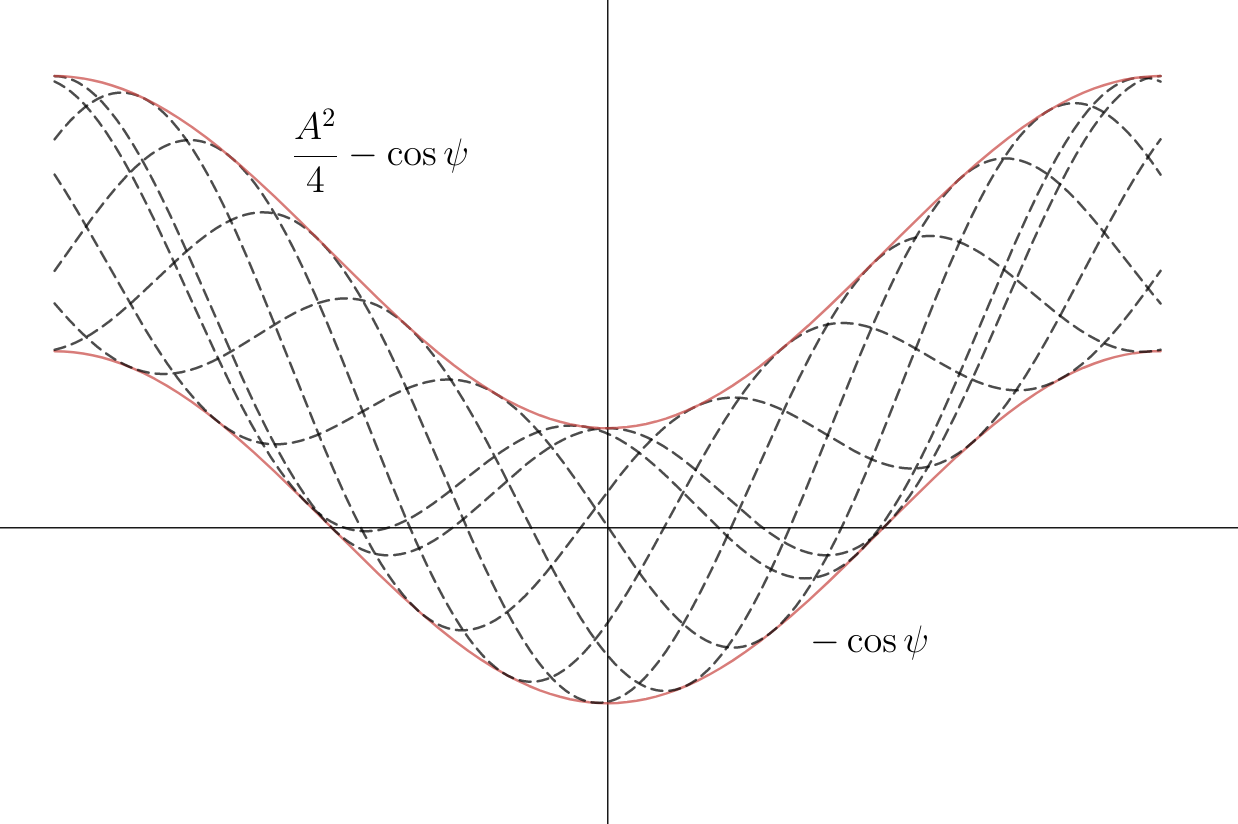
\includegraphics[scale=0.35]{limitation.png}}
		\caption{Графики зависимости $U(\psi)$ при различных $\theta$ отмечены пунктиром.}
	\end{figure}
	
	
	Понятно, что касание с ограничивающими кривыми происходит когда слагаемое $\frac{A^2}{4}\cos^2(\psi-\theta)$ обращается в $0$ или $1$.
	
	
	Детальней рассмотрим что происходит на интервалах между касаниями. Сначала положим, что $A>2$. Точки касания: $\left\{ \theta-\pi;\theta-\pi/2;\theta;\theta+\pi/2 \right\} = \left\{\psi_1,\psi_2,\psi_3,\psi_4\right\}$. 
	
	
	
	\subsubsection*{Участок $(\psi_1,\psi_2)$}На интегрвале $(\psi_1,\psi_2)$ производная $\partial U / \partial \psi < 0 $:
	\[\partial U / \partial \psi = -\frac{A^2}{4}\sin(2\psi-2\theta) + \sin \psi = \left\{\psi = t + \theta - \pi\right\} = -\frac{A^2}{4}\sin(2t)-\sin (t+\theta)\eqno(5.3.2)\]
	\[\begin{cases}
	t \in \left(0;\pi/2\right) \\
	\theta \in \left(0;\pi/2\right)
	\end{cases} \Rightarrow \begin{cases}
	\theta+t \in \left(0;\pi\right) \\
	-A^2/4\sin(2t) < 0
	\end{cases} \Rightarrow \begin{cases}
	-\sin(\theta+t) < 0 \\
	-A^2/4\sin(2t) < 0
	\end{cases} \Rightarrow \partial U / \partial \phi <0 \eqno(5.3.3)\]
	\begin{figure}[h!]
		\center{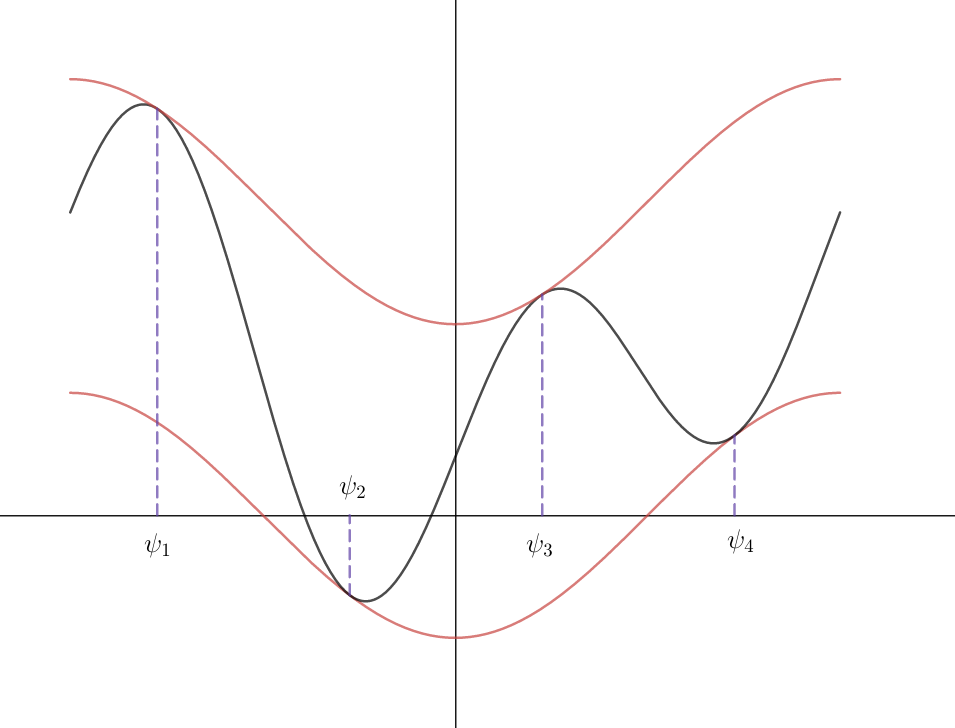
\includegraphics[scale=0.5]{segments.png}}
		\caption{Пример графика зависимости $U(\psi), A>2$}
	\end{figure}
	Важно заметить, что в рассуждениях не использовался факт $A>2$, значит вывод о знаке производной справделив при любых $A$.
	\subsubsection*{Участок $(\psi_2,\psi_3)$}
	Производные в точках $\psi_2,\psi_3$ имеют разные знаки: $\frac{\partial U}{ \partial \psi} (\psi_2) < 0\;\;\;\frac{\partial U}{ \partial \psi} (\psi_3) > 0$, действительно, ведь в точках $\psi_2,\psi_3$ член $\sim \cos^2(\psi-\theta)$ имеет нулевую производную, значит знак производной определяет $-\cos(\psi)$. Из гладкости функции потенциала делаем вывод, что производная непрерывна, а значит существует точка $\psi^* \in (\psi_2;\psi_3)$, которая отвечает минимуму потенциальной энергии.
	
	
	Покажем, что на $(\psi_2,\psi_3)$ существует только один экстремум. Для этого положим противное и выберем из набора точек экстремума $\psi*_1,\psi*_2,.. \in (\psi_2,\psi_3) $ минимальный, пусть это будет $\psi*_1 \equiv \psi_0$. Тогда для производной потенциальной энергии верно:
	\[\frac{\partial U}{\partial \psi} = -\frac{A^2}{4}\sin(2\psi-2\theta) + \sin\psi = \left\{\psi = t + \theta - \pi/2\right\} = \frac{A^2}{4}\sin(2t) - \cos(t+\theta) \eqno(5.3.4)\]
	\begin{figure}[h!]
		\center{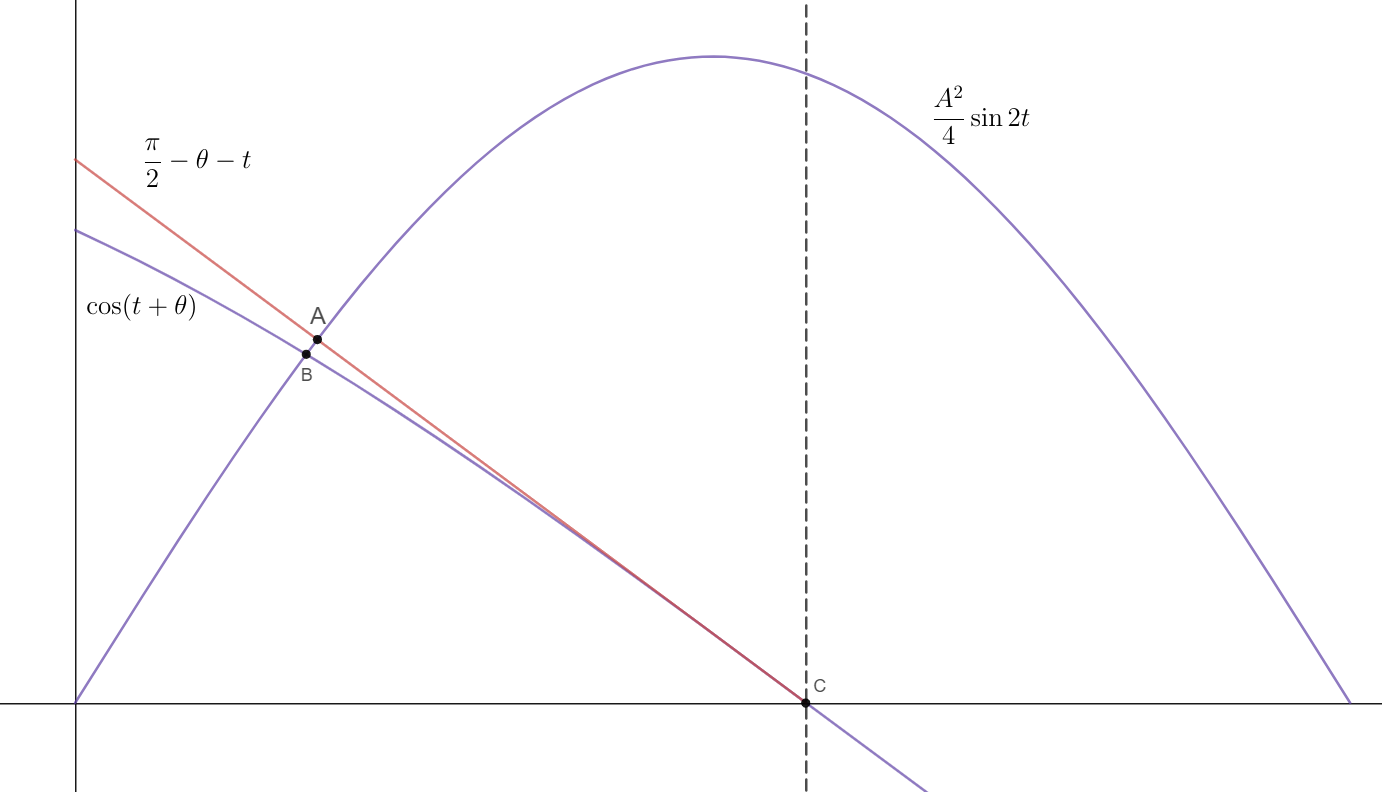
\includegraphics[scale=0.37]{displacement.png}}
	\end{figure}
	
	
	Функция $\frac{A^2}{4}\sin(2t)$ является выпуклой вверх, а это значит, что любая секущая будет лежать не выше графика. Т.е справедлива цепочка неравенств: $\cos(t+\theta) < \frac{\pi}{2} - \theta - t < \frac{A^2}{4}\sin(2t) \;\;\; \forall t \in \Big(A_t,C_t\Big)$\footnote{Тут A --- это точка на графике, а $A_t$ --- ордината точки $A$}. Причем, проверка крайних точек интегрвала показывает, что $\forall t \in \left[A_t,C_t \right]$ верно $\cos(t+\theta) < \frac{A^2}{4}\sin(2t)$. Повторяя рассуждения для интервала $\Big(B_t,A_t\Big)$, убеждаемся, что $\forall t \in \Big(B_t,C_t \Big] \;\; \cos(t+\theta) < \frac{A^2}{4}\sin(2t)$, а с учетом того, что $\frac{A^2}{4}\sin2t >= 0 > \cos(t+\theta) \forall t \in \Big(C_t,\frac{\pi}{2} \Big]$ делаем вывод: на $(\psi_2;\psi_3)$ будет только один минимум потенциальной энергии. В данном пунке никаких предположений относительно значений $A$ не выдвигалось, а значит и результат, полученный в данном пункте не зависит от $A$.
	
	
	\subsubsection*{Участок $(-\pi,\psi_1) \cup (\psi_4,\pi) $}
	Тут, как и в прошлом пункте, в крайних\footnote{Под крайними точками в данном случае мы будем понимать $\psi_1$ и $\psi_4$, т.к. объединение двух интервалов по сути описывает изменеие угла в пределах $(\psi_4,2\pi+\psi_1)$} точках знаки $\frac{\partial U}{\partial \psi}$ различны: $\frac{\partial U}{\partial \psi} (\psi_4) > 0\; \frac{\partial U}{\partial \psi} (\psi_1) < 0$. Гладкость функции потенциала позволяет нам заключить, что на данном участке есть точка максимума. Доказательство единественности и независимости от $A$ ответа можно посмотреть в прошлом пунке, ход рассуждений для данного интервала будет аналогичным.
	
	\subsubsection*{Участок $(\psi_3,\psi_4)$}
	Самый интересный участок потенциала, т.к. на данном интервале уголов количество точек равновесия зависит от параметра $A$.Разобьем интервал на два равных и посмотрим что происходи с точками равновесия. Для этого изучим знак производной в точке $\psi_3+\pi/4$:
	\[\frac{\partial U}{\partial \psi}(\psi_3+\pi/4) = \sin(\theta+\pi/4)-\frac{A^2}{4} \eqno(5.3.5)\]
	\begin{enumerate}
		\item $A > 2$, тогда для любого угла $\theta$ значение производной в центральной точке будет отрицательным, тогда мы приходим к знакомой ситуации, когда знаки производных в крайних точках интервала различны ($U'_{\psi}(\psi_3) > 0\;\;U'_{\psi}(\psi_4) > 0\;\;U'_{\psi}(\psi_3+\pi/4) < 0$). Интервал содержит 1 максимум и 1 минимум потенциальной энергии.
		\item $A = 2$, тогда при $\theta = \frac{\pi}{4}$ производная обращается в 0, но данная точка не является точкой экстремума.
		\item $A = 2$, $\theta \neq \frac{\pi}{4}$ возвращаемся к пункту 1.
		\item $\sqrt{2}<A < 2$, $\theta + \frac{\pi}{4} \in \Big[\frac{\pi}{4};\arcsin\big(\frac{A^2}{4}\big)\Big)\cup\Big( \pi -  \arcsin\big(\frac{A^2}{4}\big) ; \frac{3\pi}{4}\Big] $ производная в центральной точке будет отрицательна $\Rightarrow$ 1 пункт.
		\item $\sqrt{2}< A < 2$, $\theta + \frac{\pi}{4} \in \Big[\frac{\pi}{4};\arcsin\big(\frac{A^2}{4}\big)\Big)\cup\Big( \pi -  \arcsin\big(\frac{A^2}{4}\big) ; \frac{3\pi}{4}\Big] $ производная в центральной точке будет положительна $\Rightarrow$ точек экстремума нет.
		\item $0<A\le \sqrt{2}$ производная в центральной точке положительная при любом угле $\theta \in (0;\pi/4)$ $\Rightarrow$ точек экстремума нет.
	\end{enumerate}
	
	\subsection*{Применимость результата}\label{Resul}
	Стоит отметить,что соотношение (4.6) было получено в предположении $r_0/l \ll 1$.Это равносильно $\gamma/\omega_0 \gg A$. Действительно если по условию нам дано, что $\gamma \gg \omega_0$, то увеличение $r_0$ до величин порядка $l$ повлечет за собой рост амплитуды колебаний маятника, но с другой стороны, если обратиться к виду потенциальной кривой (см Рис.3 или Рис. 2), то становится ясно, что увеличение $A$ делает потенциальные ямы уже, а следовательно, и амплитуды колебаний меньше.

	\pagebreak
	\begin{thebibliography}{9} 
		\bibitem{variations}А.В. Ожегова, Р.Г. Насибуллин, Методические указания к решению
		"простейшей задачи" вариационного
		исчисления, Казань, 2013. 
		\bibitem{landau} Ландау Л. Д., Лифшиц Е. М. Механика. — Издание 4-е, исправленное. — Москва: Наука, 1988.
	\end{thebibliography}
	


\end{document}